\documentclass[12pt]{book}
\usepackage[utf8]{inputenc}
\usepackage[T1]{fontenc}
\usepackage{tocbibind}
\usepackage{mathptmx}
\usepackage{geometry}
\usepackage{mathtools}
\usepackage[english]{babel}
\usepackage{graphicx}
\usepackage{subcaption}
\usepackage{stackengine}
\usepackage[os=win]{menukeys}
\usepackage{hyperref}
\usepackage{xcolor}
\usepackage{color}
\usepackage{tikz}
\usepackage[yyyymmdd,hhmmss]{datetime}
\usepackage{etoolbox}
\usepackage[inline]{enumitem}
\usepackage{listings}
\usepackage{booktabs}
\usepackage[os=win]{menukeys}
\usepackage{parskip}

\newcommand{\WindowsLogo}{\raisebox{-0.1em}{
\includegraphics[height=0.8em]{images/logo/Windows_3_logo_simplified}}}
%\newcommand{\PowerLogo}{\raisebox{-0.1em}{
\includegraphics[height=0.8em]{images/logo/power}}}
\newcommand{\WinKey}{\keys{\WindowsLogo}}
\newcommand{\PowerKey}{\keys{\PowerLogo}}

%%%%% Mengganti label "Contents" ke "Daftar Isi" %%%%%
\addto\captionsenglish{\renewcommand{\contentsname}{Daftar Isi}}

%%%%% Mengganti label "Chapter" ke "Bab" %%%%%
\addto\captionsenglish{\renewcommand{\chaptername}{Bab}}

%%%%% Mengganti label "Figure" ke "Gambar" %%%%%
\addto\captionsenglish{\renewcommand{\figurename}{Gambar}}

%%%%% Mengganti label "List of Figures" ke "Daftar Gambar" %%%%%
\addto\captionsenglish{\renewcommand{\listfigurename}{Daftar Gambar}}

%%%%% Mengganti label "Table" ke "Tabel" %%%%%
\addto\captionsenglish{\renewcommand{\tablename}{Tabel}}

%%%%% Mengganti label "List of Tables" ke "Daftar Table" %%%%%
\addto\captionsenglish{\renewcommand{\listtablename}{Daftar Tabel}}

\hypersetup{
	colorlinks=true, %set true if you want colored links
	linktoc=all,     %set to all if you want both sections and subsections linked
	linkcolor=blue,  %choose some color if you want links to stand out
	urlcolor=blue,   %url color
}

\geometry{
	a4paper,
	left=10mm,
	right=10mm,
	top=15mm,
	bottom=15mm,
}

\date{}

\hypersetup{citecolor=black}

\definecolor{LightGray}{gray}{0.95}

%\pagecolor[rgb]{0.1,0.1,0.1}
%\color[rgb]{1,1,1}

\lstset
{
	language=bash,
	breaklines=true,
	basicstyle=\tt\normalsize,
	frame = single
}

\begin{document}
	\frontmatter
	\begin{titlepage}
		\centering
		{\LARGE \bf Panduan Instalasi Software Open-Source untuk Pengembangan Sistem Tertanam}
		\vfill
		{\Large Achmadi ST MT}
		\vfill
		Update: {\today}
		\vfill
		
\includegraphics[width=250pt]{images/pancasila}
		\vfill
		\vfill
		\vfill
	\end{titlepage}
	
	%%%%%%%%%%%%%%%%%%%%%%%%%%%%%%%%%%%%%%%%%%%%%%%%%%%%%%%%%%%%%%%%%
	
	\newpage
	\tableofcontents
	\listoffigures
	\listoftables
	
	%%%%%%%%%%%%%%%%%%%%%%%%%%%%%%%%%%%%%%%%%%%%%%%%%%%%%%%%%%%%%%%%%
	
	%%%%%%%%%%%%%%%%%%%%%%%%%%%%%%%%%%%%%%%%%%%%%%%%%%%%%%%%%%%%%%%%%
	
	\newpage
	\chapter{Penggunaan Buku}
	
	\section{Umum}
	Buku ini dibuat dengan tujuan penggunaan utama sebagai panduan digital untuk mempermudah search dan copy-paste.
	Anda tidak perlu mencetak buku ini ke bentuk kertas.
	Seluruh navigasi buku ini diharapkan menggunakan klik ke hyperlink di Daftar Isi,
	atau menggunakan tampilan \textbf{Index} yang tersedia di \textbf{SideBar} program pembaca PDF yang anda gunakan.
	
	\section{Petunjuk}
	Beberapa petunjuk yang digunakan di buku ini:
	\begin{itemize}
		\item \textbf{Cetak Tebal}: Menginformasikan identifier (keyword, variabel, fungsi, alamat, nama file, dst) yang berada di suatu paragraf
		\item \textbf{TIPS:} Menginformasikan hal-hal yang dapat membantu atau pengetahuan tambahan.
		\item \textbf{PERINGATAN:} Menginformasikan hal-hal yang benar-benar harus diperhatikan.
		\item Bentuk \menu[,]{File,Save} dan \keys[,]{ctrl,s} menunjukkan klik menu dan tombol keyboard.
	\end{itemize}
	
	%%%%%%%%%%%%%%%%%%%%%%%%%%%%%%%%%%%%%%%%%%%%%%%%%%%%%%%%%%%%%%%%%
	
	\newpage
	\mainmatter
	\chapter{Sistem Operasi}
	
	\section{Rekomendasi Sistem Operasi}
	
	Berikut adalah sistem operasi yang direkomendasikan dengan pertimbangan:
	
	\begin{itemize}
		\item Software terbuka menyediakan untuk lingkungan sistem operasi tersebut.
		
		\item Update untuk sistem operasi tersebut cukup dekat dengan \textit{upstream}.
		
		\item Penulis menggunakan sistem operasi tersebut secara pribadi.
	\end{itemize}
	
	\subsection{Arch Linux}
	
	Arch Linux adalah sistem operasi berbasis GNU/Linux yang bersifat sederhana dan fleksibel.
	Sistem Operasi ini dibangun untuk pengguna GNU/Linux level menengah dan seterusnya.
	Untuk pemula atau tidak mampu mencoba di lingkungan virtual/emulasi, silahkan pilih opsi lain.
	
	Berikut beberapa contoh panduan instalasi:
	
	\begin{itemize}
		\item Instalasi Arch Linux: \url{https://itsfoss.com/install-arch-linux/}.
		
		\item Instalasi Desktop (contoh Mate Desktop): \\
		\url{https://www.tecmint.com/install-mate-desktop-in-arch-linux/}
	\end{itemize}
	
	\begin{figure}[!ht]
		\centering
		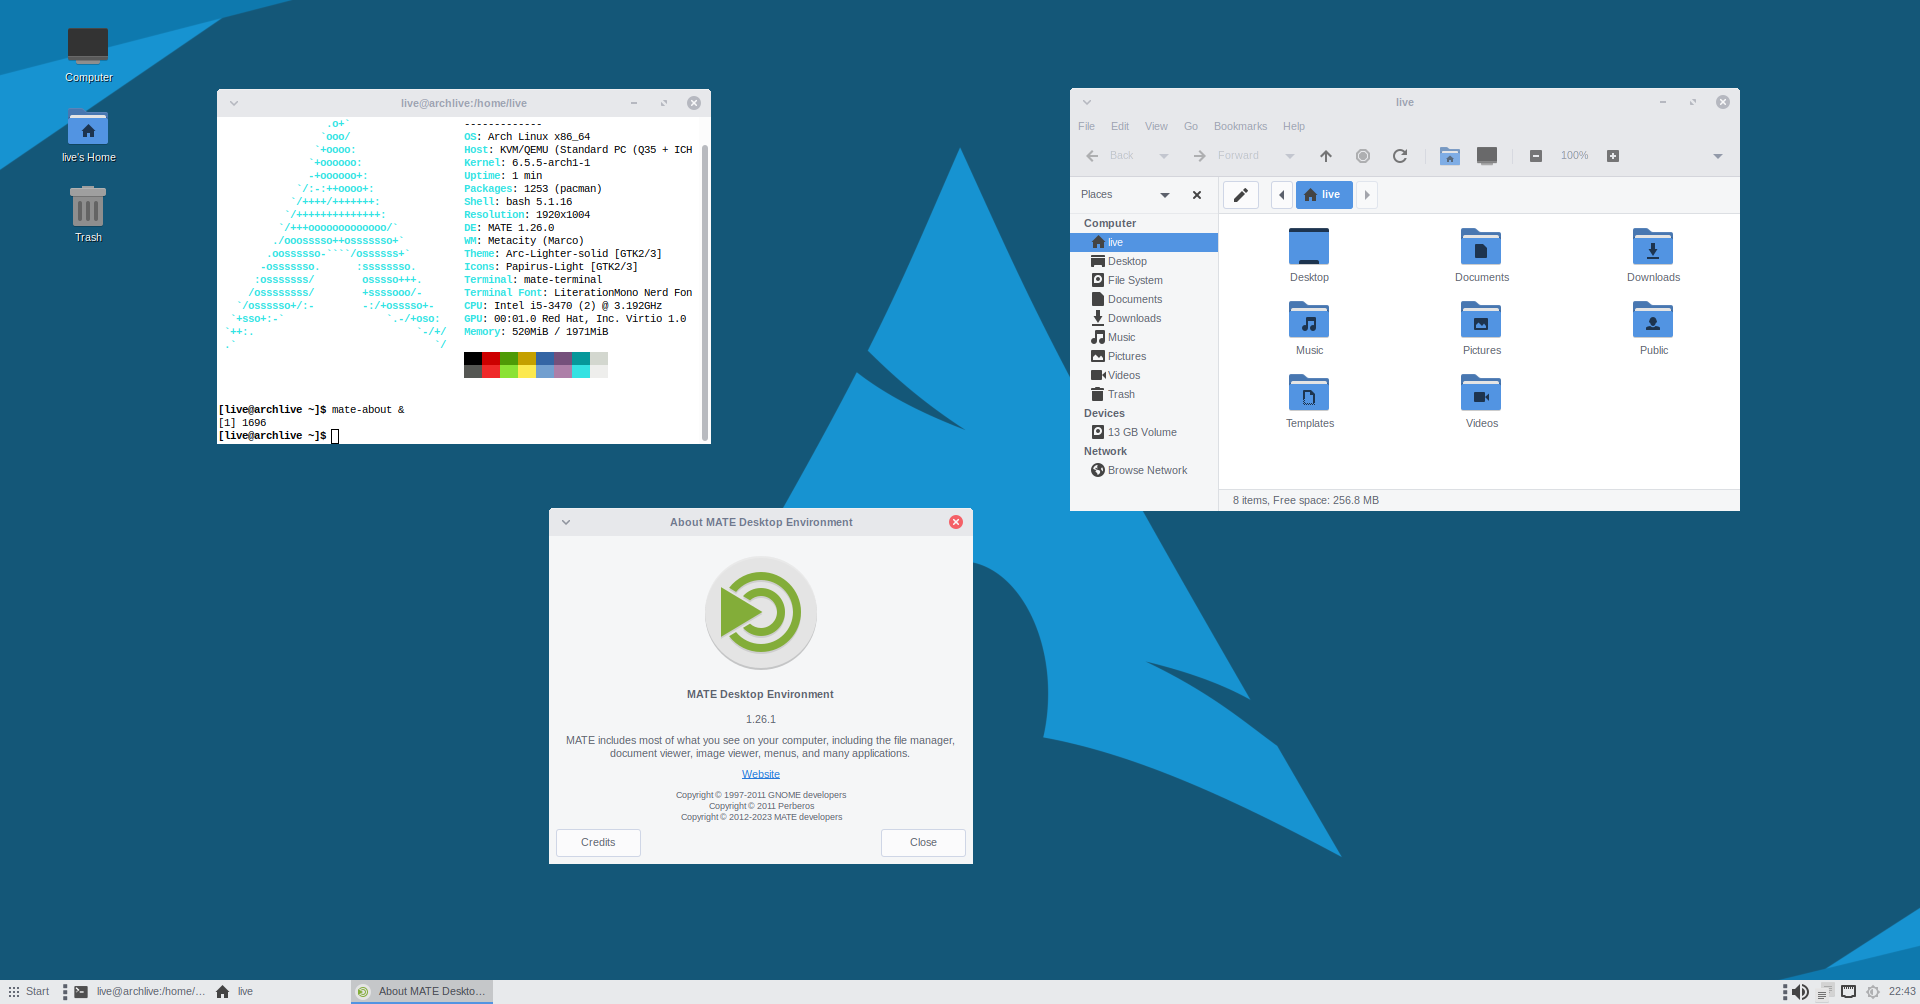
\includegraphics[width=0.8\textwidth]{images/os/archmate}
		\caption{Contoh Arch Linux}
	\end{figure}
	
	\newpage
	\subsection{Manjaro}
	
	Manjaro adalah sistem operasi turunan Arch Linux yang menyediakan image ISO yang siap install secara offline.
	Manjaro cenderung lebih ramah untuk pengguna pemula.
	
	Berikut contoh instalasi:
	
	\begin{itemize}
		\item Situs Manjaro: \url{https://manjaro.org/}
		
		\item Download ISO untuk Mate Desktop Minimal sebagai contoh: \\
		\url{https://download.manjaro.org/mate/23.0.1/manjaro-mate-23.0.1-minimal-230921-linux65.iso}
		
		\item Instalasi Manjaro: \\
		\url{https://itsfoss.com/install-manjaro-linux/}
	\end{itemize}
	
	\begin{figure}[!ht]
		\centering
		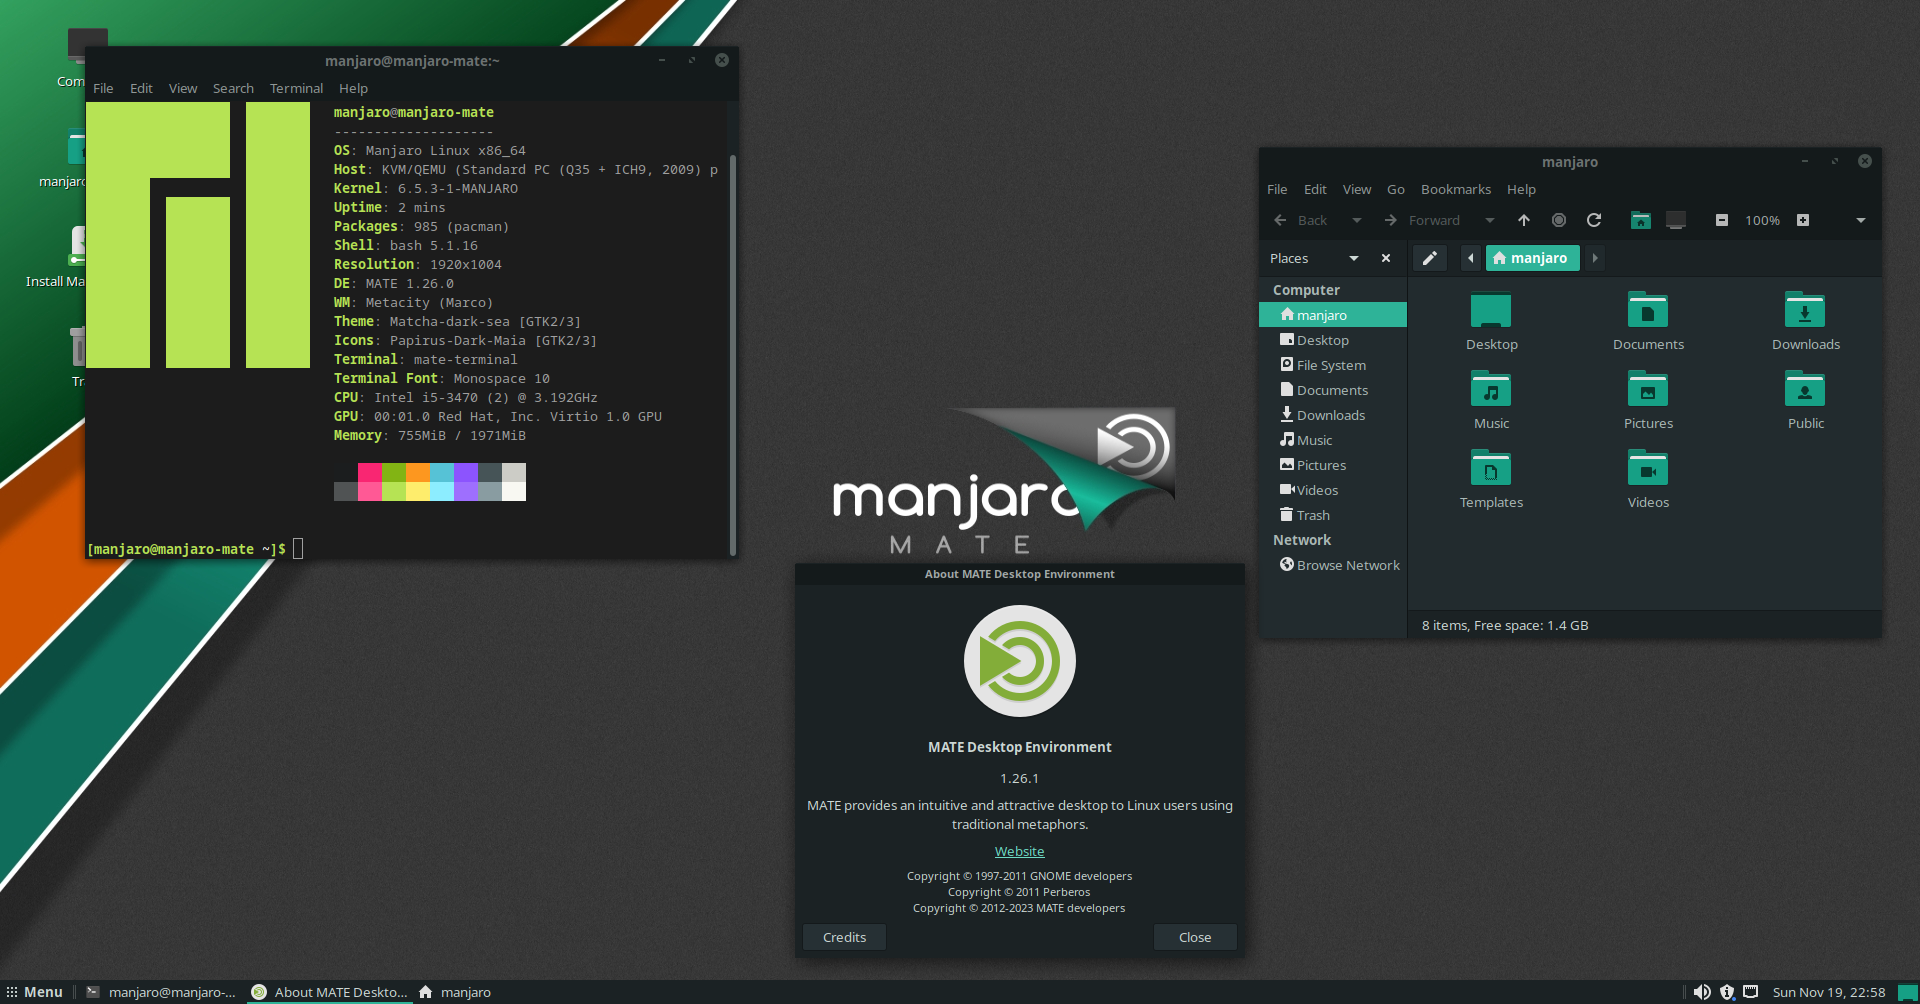
\includegraphics[width=0.8\textwidth]{images/os/manjaro}
		\caption{Contoh Manjaro}
	\end{figure}
	
	\subsection{Windows MSYS2}
\end{document}
